\chapter{Una suave introducción a GObject}
\label{oop-gobject}

En el capítulo anterior hemos aprendido a escribir código semi-orientado a objetos en C. Así es como se escriben las clases en GLib core. GObject avanza varios pasos en la programación orientada a objetos, con herencia, interfaces, funciones virtuales, etc. GObject también simplifica el paradigma de programación dirigida por eventos, con señales y propiedades.

Se recomienda crear sus propias clases de GObject para escribir una aplicación GLib / GTK. Desafortunadamente, el código es un poco detallado, porque el lenguaje C no está orientado a objetos. El código repetitivo es necesario para algunas funciones, pero no tenga miedo, existen herramientas y scripts para generar el modelo repetitivo.

Sin embargo, este capítulo da un paso atrás del capítulo anterior, es solo una pequeña introducción a GObject; explicará las cosas esenciales para saber cómo \emph{usar} una clase GObject existente (como todos los widgets y clases GTK en GIO). No explicará cómo \emph{crear} sus propias clases de GObject, porque ya está bien cubierto en el manual de referencia de GObject, y el objetivo de este libro no es duplicar todo el contenido de los manuales de referencia, el objetivo es más para que sirva de guía de introducción.

Entonces, para obtener información más detallada sobre GObject y saber cómo crear subclases, la documentación de referencia de GObject contiene capítulos introductorios: ``\emph{Conceptos}'' y ``\emph{Tutorial}'', disponibles en:

\url{https://developer.gnome.org/gobject/stable/}

Para explicar ciertos conceptos, se toman algunos ejemplos de GTK o GIO. Al leer este capítulo, se le anima a abrir Devhelp en paralelo, para mirar la referencia de API y ver por sí mismo cómo se documenta una biblioteca basada en GObject. El objetivo es que seas autónomo y puedas aprender cualquier clase nueva de GObject, ya sea en GIO, GTK o cualquier otra biblioteca.

\section{Herencia}
\label{oop-gobject-inheritance}

Un concepto importante de OOP es la herencia. Una clase puede ser una subclase de una clase principal. La subclase hereda las características de la clase padre, extendiendo o anulando su comportamiento.

La biblioteca GObject proporciona la clase base \lstinline{GObject}. Cada clase en GIO y GTK hereda, directa o indirectamente, de la clase base \lstinline{GObject}. Al mirar una clase basada en GObject, la documentación (si está escrita con GTK-Doc) siempre contiene una \emph{Jerarquía de objetos}. Por ejemplo, \lstinline{GtkApplication} tiene la siguiente jerarquía de objetos:

\begin{verbatim}
GObject
└── GApplication
    └── GtkApplication
\end{verbatim}

Significa que cuando crea un objeto \lstinline{GtkApplication}, también tiene acceso a las funciones, señales y propiedades de \lstinline{GApplication} (implementado en GIO) y \lstinline{GObject}. Por supuesto, las funciones \lstinline{g_application_*} toman como primer argumento una variable de tipo ``\lstinline{GApplication *}'', no ``\lstinline{GtkApplication *}''. Para convertir la variable en el tipo correcto, la forma recomendada es usar la macro \lstinline{G_APPLICATION()}. Por ejemplo:

\begin{lstlisting}
GtkApplication *app;

g_application_mark_busy (G_APPLICATION (app));
\end{lstlisting}

\section{Macros de GObject}

Cada clase de GObject proporciona un conjunto de macros estándar. La macro \lstinline{G_APPLICATION()} como se demostró en la sección anterior es una de las macros estándar proporcionadas por la clase \lstinline{GApplication}.

No todas las macros estándar de GObject se explicarán aquí, solo las macros útiles para \emph{usar} un GObject de una manera básica. Las otras macros son más avanzadas y generalmente son útiles solo cuando se subclasifica una clase GObject, cuando se crea una propiedad o una señal, o cuando se reemplaza una función virtual.

Cada clase GObject define una macro de la forma \lstinline{NAMESPACE_CLASSNAME(object)}, que convierte la variable al tipo ``\lstinline{NamespaceClassname *}'' y comprueba en tiempo de ejecución si la variable contiene correctamente un \lstinline{NamespaceClassname} objeto o una subclase del mismo. Si la variable es \lstinline{NULL} o contiene un objeto incompatible, la macro imprime un mensaje de advertencia crítico en la consola y devuelve NULL.

Un elenco estándar también funciona, pero la mayoría de las veces no se recomienda porque no hay comprobaciones de tiempo de ejecución:
\begin{lstlisting}
GtkApplication *app;

/* Not recommended */
g_application_mark_busy ((GApplication *) app);
\end{lstlisting}

Otra macro útil cuando se usa un GObject es \lstinline{NAMESPACE_IS_CLASSNAME(object)}, que devuelve \lstinline{TRUE} si la variable es un objeto \lstinline{NamespaceClassname} o una subclase del mismo.

% PARA HACER mostrar un ejemplo de una función que verifica sus argumentos con g_return?

\section{Interfaces}

Con GObject es posible crear interfaces. Una interfaz es solo una API, no contiene la implementación. Una clase GObject puede implementar una o varias interfaces. Si una clase GObject está documentada con GTK-Doc, la documentación contendrá una sección \emph{Interfaces implementadas}.

Por ejemplo, GTK contiene la interfaz \lstinline{GtkOrientable} que es implementada por muchos widgets y permite establecer la orientación: horizontal o vertical.

Las dos macros explicadas en la sección anterior también funcionan para interfaces. Un ejemplo con \lstinline{GtkGrid}:
\begin{lstlisting}
GtkWidget *vgrid;

vgrid = gtk_grid_new ();
gtk_orientable_set_orientation (GTK_ORIENTABLE (vgrid),
                                GTK_ORIENTATION_VERTICAL);
\end{lstlisting}

Entonces, cuando busca una determinada característica en la API para una cierta clase de GObject, la característica se puede ubicar en tres lugares diferentes:
\begin{itemize}
    \item En la propia clase GObject;
    \item En una de las clases padre en \emph{Jerarquía de objetos};
    \item O en una de las \emph{Interfaces implementadas}.
\end{itemize}

\section{Recuento de referencias}

La gestión de la memoria de las clases de GObject se basa en \emph{recuento de referencias}. Una clase GObject tiene un contador:
\begin{itemize}
    \item Cuando se crea el objeto, el contador es igual a uno;
    \item \lstinline{g_object_ref()} incrementa el contador;
    \item \lstinline{g_object_unref()} disminuye el contador;
    \item Si el contador llega a cero, el objeto se libera.
\end{itemize}

Permite almacenar el GObject en varios lugares sin necesidad de coordinar cuándo liberar el objeto.

\subsection{Evitar ciclos de referencia con referencias débiles}

Si el objeto A hace referencia al objeto B y el objeto B hace referencia al objeto A, hay un ciclo de referencia y los dos objetos nunca se liberarán. Para evitar ese problema, existe el concepto de referencias ``débiles''. Al llamar a \lstinline{g_object_ref()}, es una referencia ``sólida''. Entonces, en una dirección hay una referencia fuerte, y en la otra dirección debe haber una referencia débil (o ninguna referencia).

\begin{figure}
  \begin{center}
    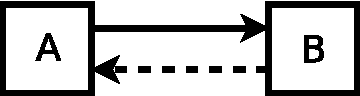
\includegraphics[scale=0.75]{assets/img/weak-ref.pdf}
    \caption{Using a weak reference to break the reference cycle between A and B.}
    \label{oop-gobject-weak-ref-schema}
  \end{center}
\end{figure}

En la Figura~\ref{oop-gobject-weak-ref-schema} podemos ver que el objeto A tiene una fuerte referencia al objeto B, y el objeto B tiene una débil referencia al objeto A.

Se puede crear una referencia débil con \lstinline{g_object_add_weak_pointer()} o \lstinline{g_object_weak_ref()}. Al igual que con las referencias fuertes, es importante liberar la referencia cuando ya no se necesite, generalmente en el destructor de clases. Una referencia débil debe eliminarse con \lstinline{g_object_remove_weak_pointer()} o \lstinline{g_object_weak_unref()}. Entonces, en la Figura~\ref{oop-gobject-weak-ref-schema}, el destructor de la clase B debe eliminar la referencia débil si aún no lo ha hecho.

\subsection{Referencias flotantes}

Cuando una clase GObject hereda de \lstinline{GInitiallyUnowned} (que es el caso de \lstinline{GtkWidget}), el objeto inicialmente tiene una referencia \emph{floating}. Se debe llamar a \lstinline{g_object_ref_sink()} para convertir esa referencia flotante en una referencia normal y fuerte.

Cuando un GObject hereda de \lstinline{GInitiallyUnowned}, significa que GObject debe incluirse en algún tipo de contenedor. El contenedor luego asume la propiedad de la referencia flotante, llamando a \lstinline{g_object_ref_sink()}. Permite simplificar el código, para eliminar la necesidad de llamar a \lstinline{g_object_unref()} después de incluir el objeto en el contenedor.

El Listado~\ref{oop-gobject-mem-management-normal} p.~\pageref{oop-gobject-mem-management-normal} muestra cómo se maneja la administración de memoria con un GObject normal. Compare esto con el Listado~\ref{oop-gobject-mem-management-floating}, que muestra cómo se maneja la administración de memoria con un GObject derivado de \lstinline{GInitiallyUnowned}. La diferencia es que \lstinline{g_object_unref()} no se llama en el último Listado, por lo que acorta el código.

\begin{lstlisting}[float=p, caption={Memory management of normal GObjects.}, label=oop-gobject-mem-management-normal]
/* Normal GObject */

a_normal_gobject = normal_gobject_new ();
/* a_normal_gobject has now a reference count of 1. */

container_add (container, a_normal_gobject);
/* a_normal_gobject has now a reference count of 2. */

/* We no longer need a_normal_gobject, so we unref it. */
g_object_unref (a_normal_gobject);
/* a_normal_gobject has now a reference count of 1. */
\end{lstlisting}

\begin{lstlisting}[float=p, caption={Memory management of GObjects deriving from \lstinline{GInitiallyUnowned}.}, label=oop-gobject-mem-management-floating]
/* GInitiallyUnowned object, e.g. a GtkWidget */

widget = gtk_entry_new ();
/* widget has now just a floating reference. */

gtk_container_add (container, widget);
/* The container has called g_object_ref_sink(), taking
 * ownership of the floating reference. The code is
 * simplified because we must not call g_object_unref().
 */
\end{lstlisting}

Entonces, es importante saber si un GObject hereda de \lstinline{GInitiallyUnowned} o no. Para eso, debe mirar la \emph{Object Hierarchy}, por ejemplo, \lstinline{GtkEntry} tiene la siguiente jerarquía:

\begin{verbatim}
GObject
└── GInitiallyUnowned
    └── GtkWidget
        └── GtkEntry
\end{verbatim}

\section{Señales y propiedades}
\label{oop-gobject-signals-and-properties}

Una clase GObject puede emitir señales. Con el bucle de eventos principal GLib (explicado anteriormente en la sección~\ref{glib-main-event-loop} p.~\pageref{glib-main-event-loop}), esta es la base para la programación dirigida por eventos. Un ejemplo de señal es cuando el usuario hace clic en un botón. La aplicación conecta una función de devolución de llamada a la señal para realizar la acción deseada cuando ocurre el evento.

Otro concepto de GObject son \emph{properties}, que está relacionado con señales. Una propiedad es básicamente una variable de instancia coronada con una señal de \lstinline{"notify"} que se emite cuando cambia su valor. Un buen ejemplo de una propiedad es el estado de un botón de verificación, es decir, un valor booleano que describe si el botón está actualmente marcado o no. Cuando el estado cambia, se envía la señal \lstinline{"notify"}.

Para crear sus propias señales o propiedades, se debe crear una subclase GObject. Como se explicó en la introducción de este capítulo, esto está más allá del alcance de este libro, pero debe tener en cuenta que, por supuesto, es posible y recomendable crear sus propias señales o propiedades. De hecho, crear una señal o propiedad de GObject es una buena manera de implementar el patrón de diseño Observer \cite{design-patterns-book}; es decir, uno o varios objetos \emph{observing} cambios de estado de otro objeto, conectando devoluciones de llamada de función. El objeto que \emph{emite} la señal no sabe qué objetos \emph{reciben} la señal. GObject solo realiza un seguimiento de la lista de devoluciones de llamada para llamar. Entonces, agregar una señal permite desacoplar clases.

\subsection{Conexión de una función de devolución de llamada a una señal}

Para hacer las cosas más concretas, si observa la documentación de \lstinline{GtkButton}, verá que proporciona la señal \lstinline{"clicked"}. Para realizar la acción deseada cuando se emite la señal, una o más funciones de devolución de llamada deben estar conectadas de antemano.

Para conectar una devolución de llamada a una señal, se puede usar la función \lstinline{g_signal_connect()}, o una de las otras funciones \lstinline{g_signal_connect_*()}:
\begin{itemize}
  \item \lstinline{g_signal_connect()}
  \item \lstinline{g_signal_connect_after()}
  \item \lstinline{g_signal_connect_swapped()}
  \item \lstinline{g_signal_connect_data()}
  \item \lstinline{g_signal_connect_object()}
  \item Y algunas más avanzadas.
\end{itemize}

El Listado~\ref{oop-gobject-gtkbutton-clicked} p.~\pageref{oop-gobject-gtkbutton-clicked} muestra el prototipo de la señal \lstinline{GtkButton::clicked} \footnote{La convención cuando se hace referencia a una señal de GObject es ``\lstinline{ClassName::signal-name}''. Así es como se documenta con los comentarios de GTK-Doc.}.

\begin{lstlisting}[float, caption={The prototype of the \lstinline{GtkButton::clicked} signal.}, label=oop-gobject-gtkbutton-clicked]
void
user_function (GtkButton *button,
               gpointer   user_data);
\end{lstlisting}

Cuando se usa \lstinline{g_signal_connect()}, la función de devolución de llamada debe tener el mismo prototipo que el prototipo de señal. Muchas señales tienen más argumentos y algunas señales devuelven un valor. Si la devolución de llamada tiene un prototipo incompatible, sucederán cosas malas, habrá errores o bloqueos aleatorios.

El Listado~\ref{oop-gobject-connect-to-signal} p.~\pageref{oop-gobject-connect-to-signal} muestra un ejemplo de cómo usar \lstinline{g_signal_connect()}.

\begin{lstlisting}[float, caption={How to connect to a signal}, label=oop-gobject-connect-to-signal]
static void
button_clicked_cb (GtkButton *button,
                   gpointer   user_data)
{
  MyClass *my_class = MY_CLASS (user_data);

  g_message ("Button clicked!");
}

static void
create_button (MyClass *my_class)
{
  GtkButton *button;

  /* Create the button */
  /* ... */

  /* Connect the callback function */
  g_signal_connect (button,
                    "clicked",
                    G_CALLBACK (button_clicked_cb),
                    my_class);
}
\end{lstlisting}

La macro \lstinline{G_CALLBACK()} es necesaria porque \lstinline{g_signal_connect()} es genérica: se puede usar para conectarse a cualquier señal de cualquier clase de GObject, por lo que el puntero de función debe ser convertido.

Hay dos convenciones principales para nombrar funciones de devolución de llamada:
\begin{itemize}
  \item Termine el nombre de la función con ``\lstinline{cb}'', atajo de `callback''. Por ejemplo: \lstinline{button_clicked_cb()} como en el ejemplo de código anterior.
  \item Inicie el nombre de la función con ``\lstinline{on}''. Por ejemplo: \lstinline{on_button_clicked()}.
\end{itemize}

Con una de esas convenciones de nomenclatura --- y con el parámetro \lstinline{gpointer user_data}, que siempre es el último parámetro --- es fácil reconocer que una función es una devolución de llamada.

El lenguaje C permite escribir una firma de función de devolución de llamada diferente --- pero compatible ---, aunque no se considera universalmente como algo bueno:
\begin{itemize}
  \item Uno o más de los \emph{últimos} argumentos de la función se pueden omitir si no se utilizan. Pero como se explicó anteriormente, el argumento \lstinline{gpointer user_data} permite reconocer fácilmente que la función es efectivamente una devolución de llamada \footnote{Al igual que con los lenguajes naturales, la redundancia permite comprender mejor y más rápidamente lo que leemos o escuchamos.}.
  \item Los tipos de argumentos se pueden modificar a un tipo compatible: p. Ej. otra clase en la jerarquía de herencia, o en el ejemplo anterior, reemplazando ``\lstinline{gpointer}'' por ``\lstinline{MyClass *}'' (pero hacer eso hace que el código sea un poco menos robusto porque \lstinline{No se llama a la macro MY_CLASS ()}).
\end{itemize}

\subsection{Desconexión de controladores de señales}

En el Listado~\ref{oop-gobject-connect-to-signal}, se llama a \lstinline{button_clicked_cb()} cada vez que el objeto \lstinline{button} emite la señal \lstinline{"clicked"}. Si el objeto \lstinline{button} todavía está vivo después de que \lstinline{my_class} se haya liberado, cuando la señal se emita nuevamente habrá un pequeño problema ... Entonces, en el destructor de \lstinline{MyClass}, el manejador de señales (es decir, la devolución de llamada) debe desconectarse. ¿Como hacer eso?

Las funciones \lstinline{g_signal_connect*()} en realidad devuelven un ID del manejador de señales, como un entero \lstinline{gulong} siempre mayor que 0 (para conexiones exitosas). Al almacenar ese ID, es posible desconectar ese manejador de señal específico con la función \lstinline{g_signal_handler_disconnect()}.

A veces también queremos desconectar el controlador de señales simplemente porque ya no estamos interesados en el evento.

El Listado~\ref{oop-gobject-disconnect-signal} muestra un ejemplo completo de cómo desconectar un manejador de señales cuando se libera su argumento \lstinline{user_data}. Volvemos a un ejemplo con un corrector ortográfico, porque el ejemplo con el botón GTK no se ajusta bien a la situación \footnote{La mayoría de las veces, un widget GTK no vive más tiempo que el contenedor al que se agrega, y el El objeto que escucha la señal del widget suele ser el propio contenedor. Entonces, si el widget muere al mismo tiempo que el contenedor, no es posible que el widget envíe una señal mientras su contenedor ya ha sido destruido. En ese caso, no tiene sentido desconectar la señal en el destructor del contenedor, ya que en ese punto el widget ya está liberado; y es más difícil para un objeto muerto enviar una señal \footnotemark.}.
% GObject es aburrido, por lo que un poco de humor no duele, una nota al pie dentro de una nota al pie, recepción al pie :-)
\footnotetext{Cuando digo que es más difícil, en realidad es imposible, por supuesto.}

El argumento de devolución de llamada \lstinline{user_data} es una instancia de \lstinline{MyTextView}, con \lstinline{MyTextView} implementado con un estilo semi-OOP. Dado que el objeto del corrector ortográfico puede vivir más tiempo que la instancia de \lstinline{MyTextView}, la señal debe desconectarse en el destructor \lstinline{MyTextView}.

\vspace{0.7cm}
\lstinputlisting[caption={Desconectar un manejador de señales cuando se libera su argumento \lstinline{user_data}.}, label=oop-gobject-disconnect-signal]{assets/code/disconnect-signal.c}

En realidad, hay otras funciones de \lstinline{g_signal_handler*()} que permiten desconectar los manejadores de señales:
\begin{itemize}
  \item \lstinline{g_signal_handlers_disconnect_by_data()}
  \item \lstinline{g_signal_handlers_disconnect_by_func()}
  \item \lstinline{g_signal_handlers_disconnect_matched()}
\end{itemize}

Habría sido posible utilizar una de las funciones anteriores en el Listado~\ref{oop-gobject-disconnect-signal}, y habría evitado la necesidad de almacenar \lstinline{word_added_to_personal_handler_id}. La función básica \lstinline{g_signal_handler_disconnect()} se ha utilizado con fines de aprendizaje.

Tenga en cuenta también que si \lstinline{MyTextView} fuera una clase GObject, habría sido posible conectarse a la señal del corrector ortográfico con \lstinline{g_signal_connect_object()}, y habría eliminado por completo la necesidad de desconectar manualmente el controlador de señal en el destructor \lstinline{MyTextView}. Una (pequeña) razón más para aprender a crear subclases de GObject.

\subsection{Propiedades}

Si ha mirado la referencia de la API GTK o GIO, debe haber notado que algunas clases de GObject tienen una o más \emph{propiedades}. Una propiedad es como una variable de instancia, también llamada ``attribute'', pero es diferente en el contexto de GObject porque tiene propiedades interesantes adicionales \footnote{Pun intencionado.}.

Como se dijo anteriormente al comienzo de la sección~\ref{oop-gobject-signals-and-properties} p.~\pageref{oop-gobject-signals-and-properties}, un buen ejemplo de una propiedad es el estado de un botón de verificación, es decir, un valor booleano que describe si el botón está actualmente marcado o no. Si ya conoce un poco de GTK, es posible que haya descubierto que hay un botón de verificación disponible con el widget \lstinline{GtkCheckButton}. Pero había una pequeña trampa si quería encontrar la propiedad de la que estaba hablando, porque la propiedad está implementada en la clase padre \lstinline{GtkToggleButton}: la propiedad \lstinline{GtkToggleButton:active} \footnote{De la misma manera Como las señales se documentan con GTK-Doc como ``\lstinline{ClassName::signal-name}'', las propiedades se documentan como ``\lstinline{ClassName:property-name}''.}.

\subsubsection{La señal \lstinline{notify} }

El atributo principal \footnote{Pun también intencionado.} De una propiedad ---~además de representar un valor~--- es que la clase GObject emite la señal \lstinline{GObject::notify} cuando cambia el valor de una propiedad.

Hay un concepto de señales GObject que aún no se ha explicado y se usa con la señal \lstinline{GObject::notify}: cuando se emite una señal, se puede proporcionar un \emph {detail}. En el caso de la señal de notificación, el detalle es el nombre de la propiedad cuyo valor ha cambiado. Dado que solo hay una señal para todas las propiedades, gracias al \emph{detail} es posible conectar una devolución de llamada para recibir una notificación solo cuando una determinada propiedad haya cambiado. Si el \emph{detail} no se proporciona al conectar la devolución de llamada, la devolución de llamada se llamará cuando \emph{cualquiera} de las propiedades del objeto cambie, lo que generalmente no es lo que se desea.

Será más claro con un ejemplo. El Listado~\ref{oop-gobject-connect-to-notify} p.~\pageref{oop-gobject-connect-to-notify} muestra cómo conectarse a la señal de notificación. Tenga en cuenta que en lugar de conectarse a la señal detallada \lstinline{"notify::active"}, en realidad es más conveniente utilizar la señal \lstinline{GtkToggleButton::toggled}. Hay mejores casos de uso en el mundo real en los que es necesario conectarse a la señal de notificación, pero al menos el Listado~\ref{oop-gobject-connect-to-notify} es, con suerte, comprensible con solo un conocimiento limitado de GTK (y si mira la documentación en Devhelp en paralelo).

\begin{lstlisting}[float, caption={Connecting to the notify signal to listen to property changes.}, label=oop-gobject-connect-to-notify]
/* If you look at the notify signal documentation, the first parameter
 * has the type GObject, not GtkCheckButton. Since GtkCheckButton is a
 * sub-class of GObject, the C language allows to write GtkCheckButton
 * directly.
 */
static void
check_button_notify_cb (GtkCheckButton *check_button,
                        GParamSpec     *pspec,
                        gpointer        user_data)
{
  /* Called each time that any property of check_button changes. */
}

static void
check_button_notify_active_cb (GtkCheckButton *check_button,
                               GParamSpec     *pspec,
                               gpointer        user_data)
{
  MyWindow *window = MY_WINDOW (user_data);
  gboolean active;

  active = gtk_toggle_button_get_active (GTK_TOGGLE_BUTTON (check_button));
  gtk_widget_set_visible (window->side_panel, active);
}

static GtkWidget *
create_check_button (MyWindow *window)
{
  GtkWidget *check_button;

  check_button = gtk_check_button_new_with_label ("Show side panel");

  /* Connect without the detail. */
  g_signal_connect (check_button,
                    "notify",
                    G_CALLBACK (check_button_notify_cb),
                    NULL);

  /* Connect with the detail, to be notified only when
   * the GtkToggleButton:active property changes.
   */
  g_signal_connect (check_button,
                    "notify::active",
                    G_CALLBACK (check_button_notify_active_cb),
                    window);

  return check_button;
}
\end{lstlisting}

\subsubsection{Vinculaciones de propiedad}

Otro aspecto útil de las propiedades es que dos propiedades se pueden vincular fácilmente: cuando una propiedad cambia, la otra se actualiza para tener el mismo valor. Lo mismo se puede lograr con la señal \lstinline{"notify"}, pero existen funciones de nivel superior.

Se pueden vincular dos propiedades de varias formas con una de las funciones \lstinline{g_object_bind_property*()}. El Listado~\ref{oop-gobject-binding-properties} muestra una implementación más simple del Listado~\ref{oop-gobject-connect-to-notify}; el código es equivalente, pero usa la función \lstinline{g_object_bind_property()}.

\vspace{0.7cm}
\begin{lstlisting}[caption={Binding two properties.}, label=oop-gobject-binding-properties]
static GtkWidget *
create_check_button (MyWindow *window)
{
  GtkWidget *check_button;

  check_button = gtk_check_button_new_with_label ("Show side panel");

  /* When the GtkToggleButton:active property of check_button changes,
   * the GtkWidget:visible property of window->side_panel is updated to
   * have the same boolean value.
   *
   * It would be useful to add G_BINDING_SYNC_CREATE to the flags, but
   * in that case the code would not be equivalent to the previous
   * code Listing.
   */
  g_object_bind_property (check_button, "active",
                          window->side_panel, "visible",
                          G_BINDING_DEFAULT);

  return check_button;
}
\end{lstlisting}